% ============================================================
%  CHAPTER 1 — INTRODUCTION
% ============================================================

In this chapter, we present the motivation for the work, the contextualization
of the problem, the main and secondary objectives, a brief literature review,
and the contributions of this TG-1, before giving an outline of the remaining
chapters.

% ------------------------------------------------------------------
\section{Motivation}

Few engineering artifacts are asked to do as much at once as an autonomous
robot.  To act well, it must turn a stream of noisy, partial measurements into
a coherent picture of its surroundings, anticipate how that picture will change,
and commit to an action before the world has finished moving.  This loop runs
continuously, under uncertainty, and with consequences that are immediate and
physical.  The same demand appears whether the robot is sorting parts on a
factory line, inspecting a pipeline on the seabed, or driving across another
planet: perceive a complex, changing world and decide what to do next.

\color{red}
figura 1: some robotics examples
\color{black}

For decades, the dominant answer to that demand was to anticipate the world on
the engineer's behalf.  Behavior was spelled out in advance as rules, state
machines, and tuned heuristics, each branch encoding a designer's expectation
of what the robot would face.  Inside a tightly controlled setting this strategy
is hard to beat.  It degrades quickly, however, as the number of situations
grows: every new contingency must be foreseen and written down by hand, the
resulting logic becomes difficult to maintain, and little of the effort carries
over when the task or the environment changes.

A different answer matured over the past decade.  Instead of prescribing
behavior, \gls{drl} lets an agent uncover it, by repeatedly acting in an
environment and adjusting toward whatever earns reward.  What makes the approach
compelling is less any single result than the steadily widening class of
problems it can absorb --- and the way those problems can be ordered by how
closely they resemble the physical world a robot inhabits.

At the structured extreme sit fully observable, turn-based games with discrete
moves.  Go is the canonical example: a player sees the entire board, acts only
on their turn, and chooses among a finite set of legal moves, yet the game hides
on the order of $10^{170}$ positions behind those simple rules.  In 2016
AlphaGo became the first program to defeat a professional human
player~\cite{silver2016mastering}, and its successor AlphaGo Zero reached the
same standard learning purely from self-play, without a single human game as a
reference~\cite{silver2017mastering}.

%% FIGURE SUGGESTION 1: AlphaGo — the Lee Sedol match photograph (2016).
%% Widely available under press license from DeepMind; cite the original source.

Relaxing those assumptions one at a time brings the setting closer to robotics.
Let many agents act simultaneously, in continuous time, while hiding part of the
state from each of them, and the difficulty changes in kind rather than degree.
AlphaStar reached this regime in StarCraft~II, where an agent must interleave
long-horizon economic planning with split-second control over individual units,
select among roughly $10^{26}$ actions at every step, and do so without ever
observing the full board~\cite{starcraft_marl}.  Tellingly, its robustness did
not come from optimizing against a single adversary but from training inside a
\emph{league} of continually evolving rivals, so that no one exploitable
strategy could survive.

\begin{figure}[h]
    \centering
    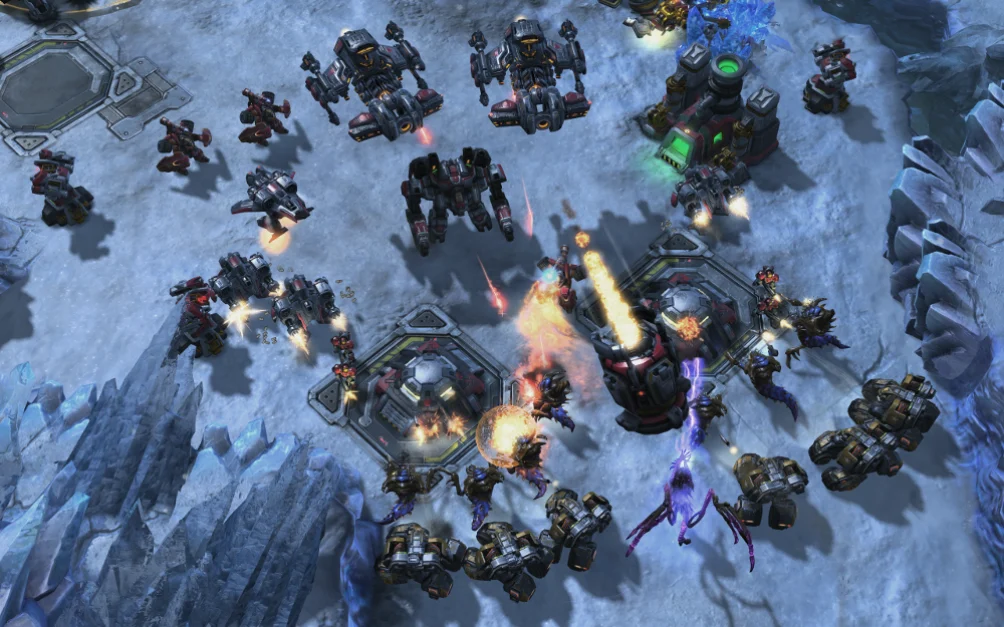
\includegraphics[width=0.8\textwidth]{Cap1/starcraft2.png}
    \caption{A picture of the StarCraft 2 game. Its possible to see a clash between units of Zerg and Terran factions. Credit: Blizzard Entertainment (\url{https://blizzard.com/}).}
    \label{fig:starcraft_2_game}
\end{figure}

What every one of these results leaves untouched, however, is the body.  A
simulated agent issues an action and the action simply happens; a physical one
must produce torques that move mass, manage balance and contact, and recover
when the world reacts in ways no rule foresaw.  This last frontier --- continuous
sensorimotor control on real hardware --- is where progress is now most striking.
Fittingly for a World Cup year, Boston Dynamics has recently demonstrated its
Atlas humanoid performing soccer skills that demand exactly this kind of
dynamic, whole-body coordination on real hardware.

\begin{figure}[h]
    \centering
    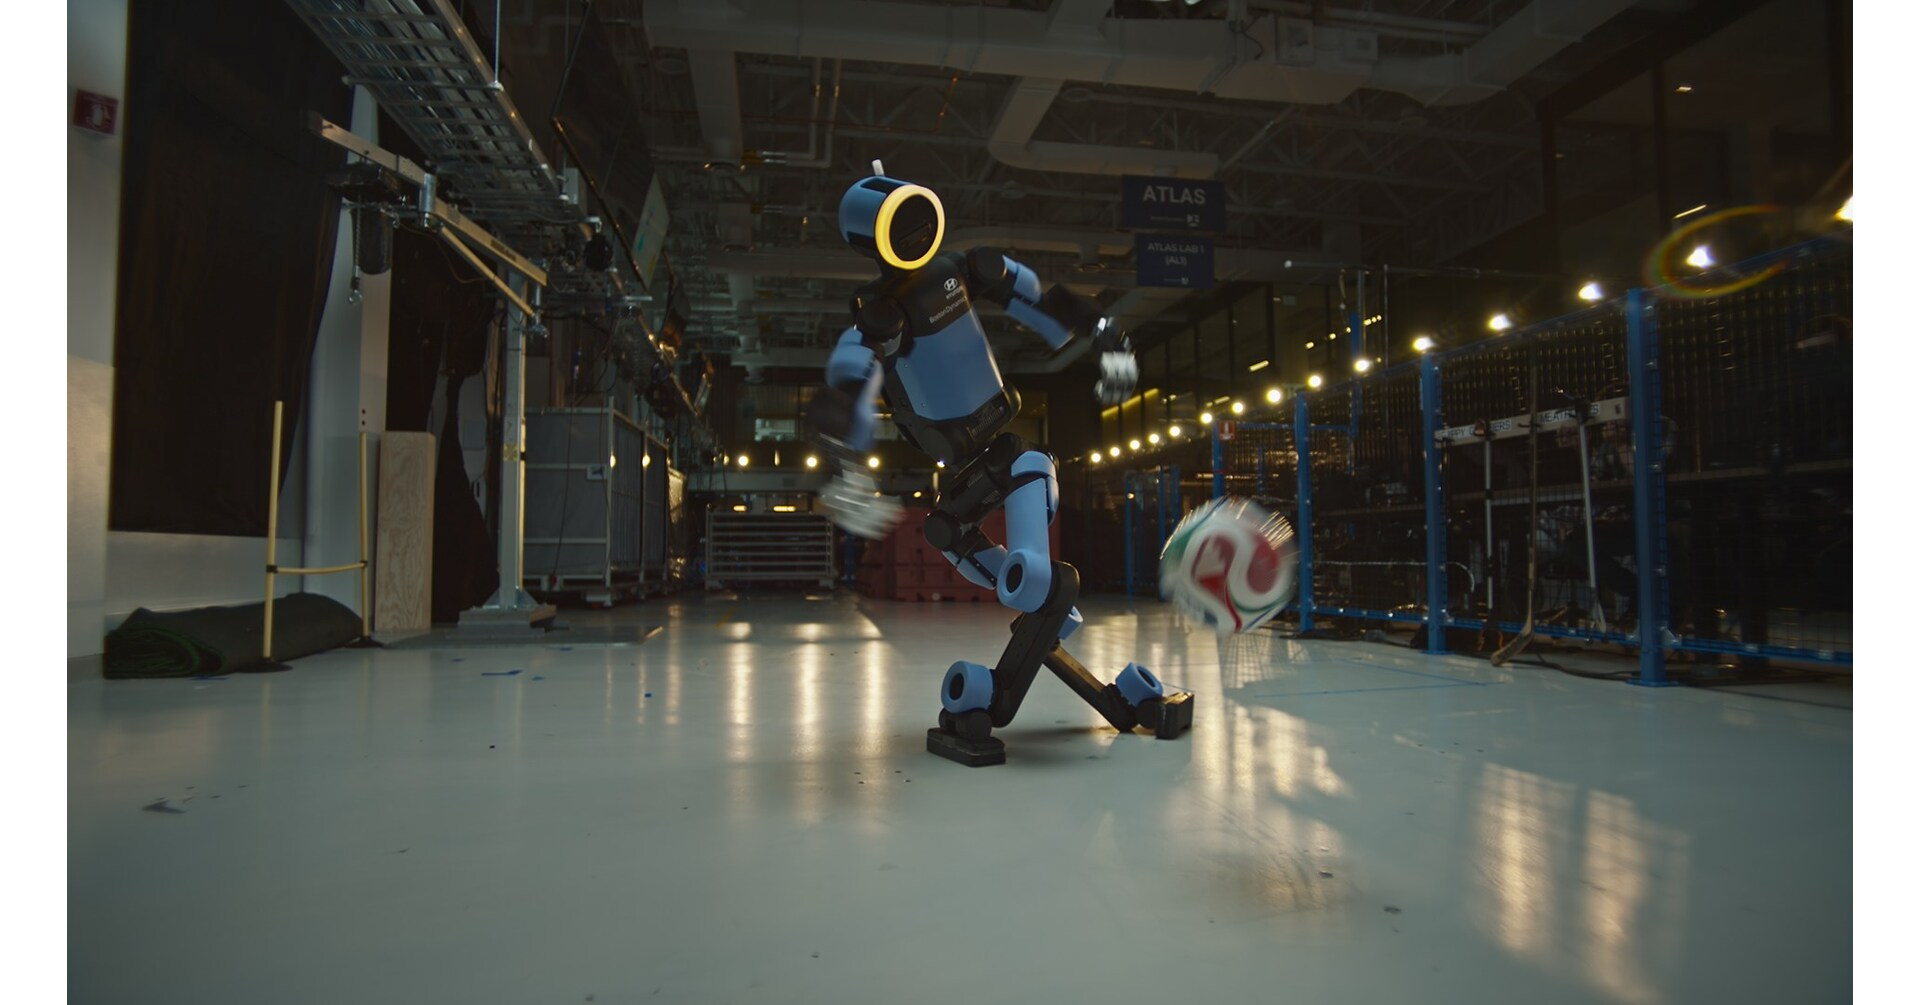
\includegraphics[width=0.8\textwidth]{Cap1/atlas_rabona.png}
    \caption{Picture of a pre-World Cup 2026 marketing stunt for the Boston Dynamics Atlas robot.
    The robot can be seen doing a "Rabona", also known as "chute de letra" in Portuguese.
    Credit: Hyundai and Boston Dynamics (\url{https://bostondynamics.com/atlas}).}
    \label{fig:atlas_rabona}
\end{figure}

Robot soccer occupies a particularly attractive position in this landscape.
It draws together, in one compact and well-defined domain, the threads pulled
apart above: continuous control, real-time decision-making, multi-agent
cooperation, and adversarial competition.  It is cheap enough to simulate at
scale, yet the underlying decision problem remains genuinely hard --- which is
precisely what makes it a demanding benchmark for techniques whose ultimate
target is the physical world.

% ------------------------------------------------------------------
\section{Contextualization}
% ------------------------------------------------------------------

In the context of Robot Soccer, various robotics leagues and competitions have surged in the last decades.
One of the popular leagues in Brazil is the IEEE Very Small Size Soccer (\gls{vsss}),
category in which two teams of
differential-drive robots play on a flat field.  A camera mounted above the
field estimates the positions of all robots and the ball; an off-board computer
processes these estimates and sends wheel-speed commands to each robot via
radio.  In the 3v3 format considered here, each team has three homogeneous
robots and no kicking mechanism, so effective team behavior must arise from
ball conduction, positioning, and coordinated movement.
Figure~\ref{fig:vsss_game_diagram} shows the common IEEE VSSS game setup.

\begin{figure}[ht]
    \centering
    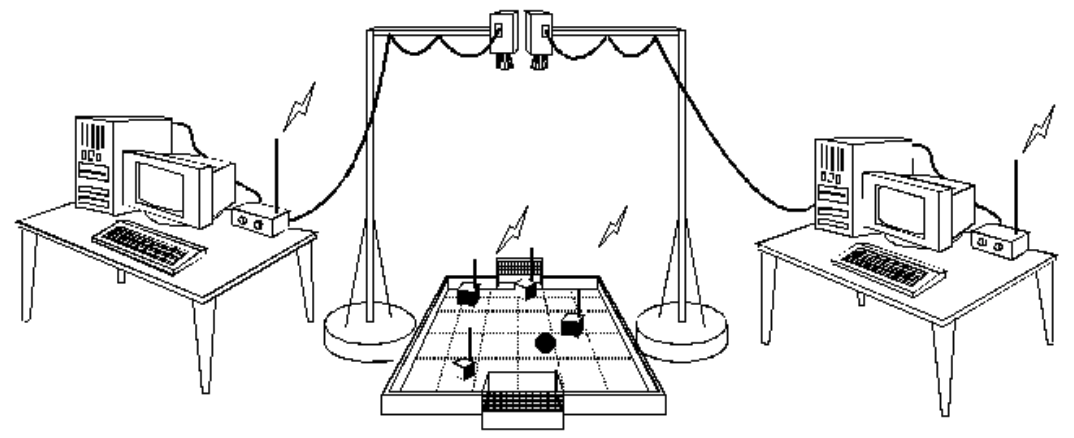
\includegraphics[width=0.82\linewidth]{Cap1/vsss_game.png}
    \caption{IEEE VSSS game set. Credit:~\cite{ieee_vsss_rules}.}
    \label{fig:vsss_game_diagram}
\end{figure}

The ITAndroids \gls{vsss} team currently relies on a classical robotics stack
for strategy, path planning, and low-level control — a hierarchy of carefully
hand-crafted rules and heuristics that govern how each robot navigates the
field and responds to game events. Figure~\ref{fig:vss_robots} shows a picture of the ITAndroids robots and the overhead-vision marker. This stack performs well in practice but
has fundamental limitations.  Rule-based strategies are designed for a finite
set of anticipated situations and do not automatically improve with more
data or competition experience.  Adapting them to a new opponent or a changed
team composition requires manual re-engineering.

\begin{figure}[ht]
    \centering
    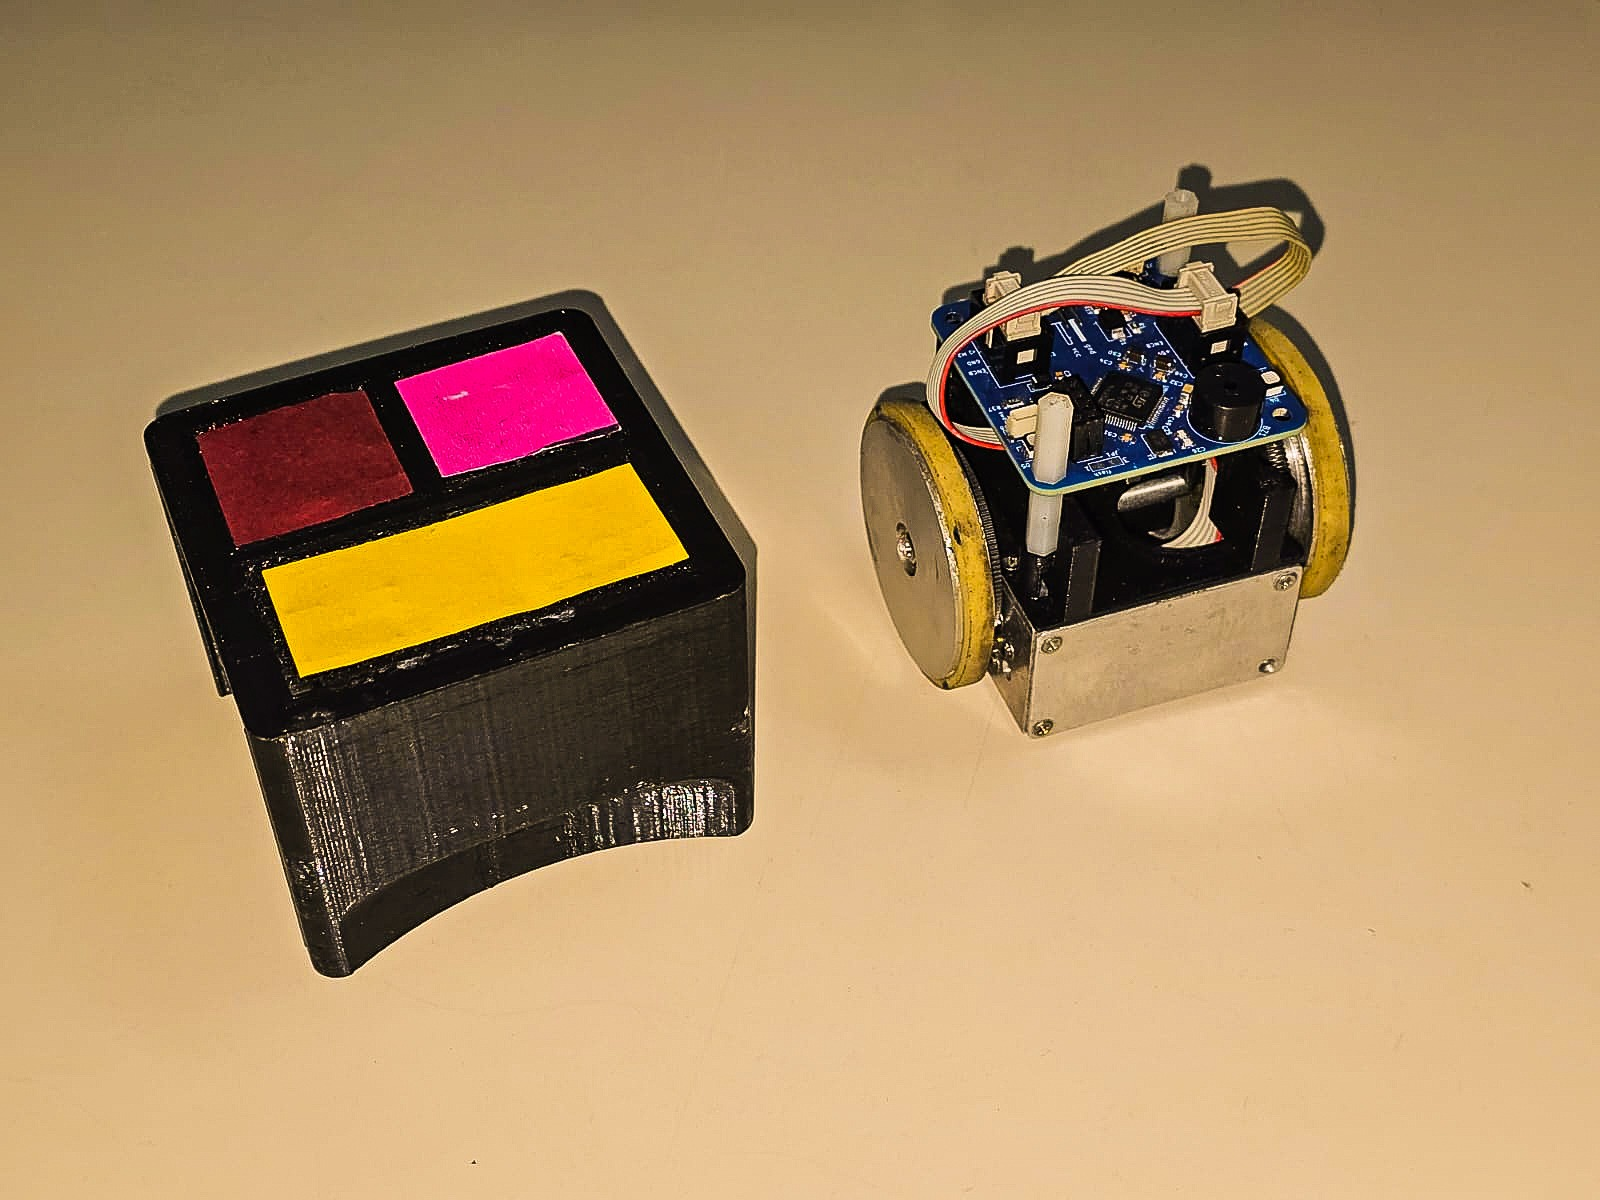
\includegraphics[width=0.75\textwidth]{Cap1/vss.jpeg}
    \caption{ITAndroids \gls{vsss} robots and overhead-vision marker.}
    \label{fig:vss_robots}
\end{figure}

The potential of learned strategies for this domain has been demonstrated by
a series of prior works, each addressing a different scope. \textcite{bassani2020}
developed an open RL framework for \gls{vsss} and showed that
a trained single-agent policy could match the level of human-designed
strategies, reaching fourth place at the 2019 Latin American Robotics
Competition (LARC). \textcite{medeiros2020} applied Proximal Policy Optimization (\gls{ppo})
with curriculum learning to teach a single robot to intercept the ball in the
presence of an opponent, outperforming both handcrafted baselines and agents
trained without the curriculum.  \textcite{tg_thay} extended
this framework to penalty kicks, achieving conversion rates substantially above
the team's existing kicker.  Subsequent work by \textcite{master_thay} moved to an adversarial multi-agent setting, studying how
different opponent-sampling strategies affect the quality of the learned policy
in penalty-kick scenarios.  \textcite{brandao2022} went
further, applying \gls{ppo} with self-play to a full 3v3 team, simultaneously
learning control and strategy, and demonstrating that the resulting policy
could defeat the best available heuristic opponent with an 84\% win
rate.

This thesis is the natural next step in that line of work.  Where \textcite{brandao2022}
showed that 3v3 multi-agent learning is feasible, the
experiments there were constrained by the cost of collecting enough useful
experience.  The central question this work addresses is what becomes possible
when training can both generate more transitions per wall-clock second and make
better use of the situations it samples.

% ------------------------------------------------------------------
\section{Objective}
% ------------------------------------------------------------------

The objective of this work is to reduce one of the main practical barriers that
still separates reinforcement-learning research in \gls{vsss} from routine use
inside the ITAndroids development cycle.  The team already has a sequence of
works showing that learned policies can perform meaningful soccer behaviors,
from isolated skills to complete 3v3 control.  However, training and evaluating
these policies remains expensive: each experiment requires a large number of
simulated interactions, and the existing simulator architecture limits how
quickly those interactions can be produced.

This work therefore concentrates on the infrastructure needed to make such a
strategy learnable.  An accelerated \gls{vsss} simulator is developed and
integrated into an end-to-end \gls{ppo} training loop for a centralized joint
team policy.  The resulting baseline allows the simulator to be measured in a
real learning setting and establishes the foundations for the sample-selection
and multi-agent extensions that follow in TG-2.

% ------------------------------------------------------------------
\section{Literature Review}
% ------------------------------------------------------------------

This section reviews the work most relevant to a learning-based approach to
3v3 \gls{vsss}.  It proceeds from the broad milestones that established deep
reinforcement learning as a viable tool for strategic control, through the
specific body of \gls{vsss} research developed within the ITAndroids team, to
accelerated simulation and sample efficiency improvements.

\subsection{Deep Reinforcement Learning in Games and Robotics}

The modern interest in deep reinforcement learning for sequential
decision-making was catalyzed by a sequence of results in games of increasing
complexity.  AlphaGo defeated a professional Go player by combining
deep neural networks with Monte Carlo tree search~\cite{silver2016mastering},
and its successor AlphaGo Zero reached superhuman play through self-play
alone, learning without any human game data~\cite{silver2017mastering}.  These
results established two ideas central to this work: that a single learned
function can encode sophisticated strategy, and that self-play can generate the
training signal needed to reach it.

Subsequent work scaled these ideas to real-time, multi-agent, partially
observable settings.  OpenAI Five coordinated a team of five agents to defeat
human champions at the video game Dota~2~\cite{berner2019dota}, and AlphaStar
reached Grandmaster level in StarCraft~II by training a league of continually
adapting agents, each representing a distinct strategy, to prevent the policy
from overfitting to a single style of play~\cite{starcraft_marl}.  The
league-training idea — that competitive robustness requires facing a diverse
population of opponents rather than only the latest policy — directly informs
the self-play design considered in this work.

\subsection{Reinforcement Learning in IEEE VSSS}

Within the \gls{vsss} category specifically, a focused body of work — much of it
produced within the ITAndroids team — has progressively expanded the role of
reinforcement learning from isolated skills toward full-team play.

\textcite{medeiros2020} introduced reinforcement learning to \gls{vsss} strategy
by training a single robot, with \gls{ppo}, to intercept and control the ball in
the presence of an opponent.  Two design choices from that
work recur throughout the subsequent literature and in this thesis.  First, the
action space was taken as the robot's wheel speeds rather than a target position
handed to an external controller, which forces the policy to solve the planning
and control problems jointly.  Second, because goal events are too sparse to
drive early learning, the reward was shaped with intermediate terms and training
was organized as a curriculum, with the agent and ball beginning close together
and gradually separating and the opponent initially stationary and later set in
motion.  Agents trained with this curriculum matched or outperformed both agents
trained without it and the team's classical heuristics, establishing \gls{ppo}
with curriculum learning as a strong baseline for the domain.

\textcite{master_thiago} later extended this framework, broadening
from a single defensive skill to four scenarios — intercepting the ball on the
player's side and recovering it to the opponent's side, each with and without an
opponent — and introducing cooperative self-play, in which each agent carries a
copy of the same network and learns to coordinate with itself rather than treat
its copy purely as an adversary. This is, to the author's
knowledge, the first work to combine self-play with \gls{ppo} in \gls{vsss}, and
its scenario-based curriculum and shared-network design are direct antecedents
of the two-stage, symmetry-aware approach taken here.

\textcite{tg_Yamane} addressed a different role and a different challenge: a learned
goalkeeper policy and, crucially, its transfer to physical
hardware.  Where the earlier works evaluated policies only in
simulation, this thesis confronts the reality gap between the simulator and the
real robot, treating line-following control and decision-making under real
sensing and actuation noise.  Its treatment of sim-to-real transfer frames the
domain-randomization and noise-injection considerations that the present work
defers to its own future-work agenda.

\textcite{master_thay} moved the framework into an explicitly adversarial,
multi-agent regime, studying penalty-kick scenarios in which an attacker and a
goalkeeper are trained against each other.  The central
question of that work is how to choose the opponent during self-play.  It
formalizes a family of opponent-sampling strategies that differ in how much of
the training history they draw from — for instance, sampling uniformly from all
past versions of the opponent, from only the most recent half, or from a fixed
recent window — and analyzes how this choice affects the robustness and quality
of the learned policy.  This is precisely the design space that the second
curriculum stage of the present work must navigate, and Baldão's analysis is the
most directly applicable guidance available for it.

Beyond the ITAndroids line, \textcite{bassani2020} developed an open
reinforcement-learning framework for \gls{vsss} and demonstrated sim-to-real
transfer of trained policies, with a resulting team placing competitively at the
2019 Latin American Robotics Competition.  Closest in spirit
to this thesis, \textcite{brandao2022} trained a full 3v3 team with multi-agent
\gls{ppo} and self-play, using a shared policy across the three homogeneous
robots and a centralized data-collection scheme, and reported a policy capable
of defeating the strongest available heuristic opponent.
That work establishes that full-team 3v3 learning is feasible; the present
work takes that feasibility as its starting point and asks what becomes possible
once the simulation-throughput and sample-efficiency constraints under which it
operated are relaxed.

\subsection{Accelerated Simulation for Reinforcement Learning}

On-policy algorithms such as \gls{ppo} consume a large volume of fresh
environment transitions, which makes simulation throughput a primary determinant
of training cost.  The \gls{vsss} works above run physics on the \gls{cpu} and
communicate with the learner across a process boundary, an architecture whose
throughput scales poorly with the number of parallel environments.

A recent direction addresses this by relocating the environment onto the
hardware accelerator.  Frameworks such as Brax express rigid-body physics as
differentiable, batched array operations that execute on \gls{gpu}, allowing
thousands of environments to be stepped simultaneously and bringing the
simulator and the learner onto the same device~\cite{brax2021}.  In the robot
soccer context specifically, \textcite{scaling_marl_2d} built a custom 2D environment
whose physics is expressed as simple vectorizable operations and reported
throughput one to two orders of magnitude higher than a wrapped general-purpose
simulator for the same task, demonstrating that a purpose-built
batched environment can dramatically reduce training time precisely because it
avoids the overhead of a general engine.  The simulator developed in this work
follows this paradigm, applying it to the \gls{vsss} domain.

\subsection{Prioritized Experience and Scenario Selection}

A complementary way to reduce training cost is to improve the value of each
transition rather than the rate at which transitions are produced.  Prioritized
Experience Replay~\cite{schaul2016per} established that, in off-policy learning,
replaying transitions in proportion to their temporal-difference error learns
faster than uniform replay.  Prioritized Level Replay (\gls{plr}) extends this
intuition to the selection of \emph{which situations to play} rather than which
past transitions to revisit: it scores environment configurations by an estimate
of their future learning potential and biases the agent's experience toward the
configurations expected to be most informative, inducing an implicit curriculum
without any predefined ordering of difficulty~\cite{prioritized_level_replay}.  The sampler
proposed in this work adapts this principle to \gls{vsss}, treating each
initialized game situation as a level whose priority is derived from the
policy's recent value-prediction error.

The same selection problem also appears in multi-agent self-play.  AlphaStar's
league training, for example, did not train only against the latest policy; it
maintained a population of agents so that the learner faced varied opponents and
did not overfit to a single strategy~\cite{starcraft_marl}.  In this work,
\gls{plr} addresses the analogous question on the environment side: which game
situations should the current policy experience next?

% ------------------------------------------------------------------
\section{Contributions}
\label{sec:contributions}
% ------------------------------------------------------------------

This work is organized around two costs that limit large-scale reinforcement
learning in \gls{vsss}: throughput, or how many fresh transitions can be
produced per second, and sample efficiency, or how informative those transitions
are for the current policy.  The first cost is addressed directly by moving the
simulator onto the accelerator.  The second is addressed in TG-1 by establishing
the training baseline and initialization interface on which the
prioritized-level-replay sampler will operate in TG-2.

The two main TG-1 contributions are therefore:

\begin{itemize}
    \item A JAX-based, GPU-parallel simulator for 3v3 \gls{vsss}, built
    around batched physics and accelerator-friendly rollout loops.  The
    simulator is designed to step thousands of independent game instances
    simultaneously on a single device, eliminating the inter-process
    communication overhead present in all existing \gls{vsss} training
    pipelines.

    \item A policy-training baseline for sample-efficient extensions: a
    centralized joint policy
    trained from scratch to control a 3v3 \gls{vsss} team using the new
    simulator, with learning curves showing that the infrastructure supports
    reliable policy improvement and characterizing the role of initialization
    strategy in the learning process.  These results motivate the
    \gls{plr} sampler and provide the comparison point for its TG-2 evaluation.
\end{itemize}

The TG-1 policy is deliberately centralized: a single network observes the
global game state and commands all three allied robots simultaneously.  This
controlled baseline isolates the throughput and sample-selection contributions
from the additional complexity of per-robot decentralization, full self-play,
and symmetry-aware data augmentation.

This work also contributes to the relatively limited literature on applying
deep \gls{rl} to full-team decision-making and control in the IEEE \gls{vsss}
league, and aligns with the ITAndroids team's mission of advancing and
disseminating knowledge in robotics and artificial intelligence.

% ------------------------------------------------------------------
\section{Outline of this Work}
% ------------------------------------------------------------------

The remainder of this work is organized as follows:
\begin{itemize}
  \item \textbf{Chapter~2} describes the IEEE \gls{vsss} domain, the differential-drive robot model, and the existing simulators used in the community and their limitations for large-scale \gls{rl} training.
  \item \textbf{Chapter~3} covers the machine-learning background: reinforcement learning fundamentals, \gls{ppo}, curriculum learning, prioritized level replay, multi-agent self-play, symmetry exploitation, and GPU-accelerated simulation.
  \item \textbf{Chapter~4} defines the proposed methodology, including the multi-agent \gls{mdp} formulation, policy architecture, and simulator design.
  \item \textbf{Chapter~5} reports preliminary TG-1 results, focusing on measured simulator throughput, interface validation and two simple example policy training experiments, as well as some of the discussion regarding the role of planned improvements in TG-2.
  \item \textbf{Chapter~6} summarizes TG-1 and defines the roadmap toward TG-2.
\end{itemize}